% !TeX spellcheck = en_US
\documentclass[a4paper]{llncs}


\usepackage{graphicx}
\graphicspath{{./images/}}
\usepackage{float}
\usepackage{amssymb}

%opening
\title{Personalized music search based on graph embedding}
\author{Christian Esswein}
\institute{christian.esswein@student.uibk.ac.at}

\begin{document}
	
	\maketitle
	
	\begin{abstract}
		While exploring new music, users are typically limited to recommender systems which are proposing items either based on their listening history or on content similarities. Combining both methods models a “query-based recommendation” which enables users to filter content based on their preferences.
		The ecosystem of music can be represented as an heterogeneous graph using all available data about users, tracks, artists, genres, tags, … . Using graph embedding techniques a low-dimensional vector representation is learned and provide simple method to calculate similarities. Search queries, either single terms or combinations of items in the music graph, can be encoded using the same vector space. Therefore, not only exact results are found, but also similar items.
		
		
		The goal of this thesis is to use graph embedding techniques for creating a latent representation of the Spotify music dataset. This low-dimensional vector embedding is used to provide personalized recommendations based on arbitrary search queries. After providing the first search results, the user should be assisted while exploring the results and in the refinement of his search terms. Instead of a list, the learned vector representation should be exploited to generate 3D representations of the suggested items.
		
		
	\end{abstract}
	
	\section{Introduction}
	While exploring new music, users are typically limited to recommender systems which are proposing items either based on their listening history or on content similarities (aka find similar artists, songs). Combining both methods models a “query-based recommendation” which enables users to filter content based on their preferences.
	The ecosystem of music can be represented as an heterogeneous graph using all available data about users, tracks, artists, genres, tags, … . Using graph embedding techniques a low-dimensional vector representation is learned and provide simple method to calculate similarities. Search queries, either single terms or combinations of items in the music graph, can be encoded using the same vector space. As a result, not only exact results are found, but also similar items.
	
	The goal of this thesis is to embed the Spotify dataset into a latent representation to enable recommendations based on queries. After providing the first search results, the user should be assisted while exploring the results and in the refinement of his search terms. Traditional list based aggregations of search results can only model a one dimensional similarity for the items. Instead of a list, the low-dimensional vector representation should be exploited to generate 3D representations of the suggested items. Combined with the graph representation, query suggestions can be provided.
	
	
	Spotify...
	\cite{aboutSpotify} Active users: Over 140 million (as of June 2017)
	Number of songs: Over 30 million
	
	Challenges of music search
	Through streaming services huge music databases are available for users. Primary objective for user is mainly not to find specific songs but to find songs matching seeding criteria. Similar songs to / similar to this artist / genre / tags. When using naive approaches with simple attribute matching complete annotated metadata is required. Otherwise song can not appear when querying for tag it has not assigned to. Especially when it comes to genres and tags it is unfeasible to manually annotate every entity. Additionally the assignment of scores is a hard task --> how to compare. having / not having. Approaches try to predict tags through audio features -> lack to compare different seeds. how to compare artists with tracks
	
	Desired search engine needs to learn representation. tags in training phase but while predicting new connections have to be drawn.
	
	
	
	
	\section{Related work}
	
	music search \cite{chen2016query}
	
	3D interface
	
	
	\section{Graph Embedding}
	Graph embedding techniques aiming to transform graph structures into low a dimensional vector space. More formally, given a graph $ G = (V,E) $ with vertices $ V $ and edges $ E $ "a graph embedding is a mapping $ f : v_{i} \rightarrow y_{i} \in \mathbb{R}^{d} $ $ \forall i \in [n] $ such that $ d \ll |V| $ and the function $ f $ preserves some proximity measure defined on graph $ G $ "\cite{goyal2017graph}.
	Advantages are to have a coherent search space for diverse element types. Embedding can be used for easy higher-order proximity calculation. Similar items should be near in vector space.
	
	Existing embedding algorithms can be categorized into factorization based, random walk based and deep walking based methods. Time complexity and properties which are preserved mainly random walk base methods are interesting ($ O(|V|) $). Here DeepWalk and node2vec are two examples both 
	
	
	Through advances in the field of natural language processing in the recent years...
	
	both node2vec and deepwalk are making use use word2vec a popular method to 
	
	
	random walks ---
	
	Deepwalk:
	\cite{perozzi2014deepwalk}
	Uses short random walks over edges to generate sentences and therefore constructs an artificial language based on the graph structure. Word2Vec is used in the reference implementation to 
	
	
	
	\subsection{Model extension}
	In real world scenarios the dataset is not fixed and during runtime more data is collected which needs to be included into the model. New data can either consists of new edges, e.g. new user-track relations produced by playing history, but also of new vertices when tracks or users are added. Especially if new users do not suffer from the cold start problem because initial data is available (eg through connecting with other services, see \ref{sec:impl_spotify_connect}), a fast method is desirable. A naive approach could simply recreate the whole embedding, but this is not scalable for bigger sets. 
	
	The random walk based embedding techniques are mostly online algorithms which can consume new walks as they are produced. This property is very powerful in general because for huge datasets not all walks have to be generated in advanced or even kept in memory. Unfortunately both reference implementations for \emph{node2vec} and \emph{DeepWalk} do not provide interfaces to store the internal state, retrieve intermediate embeddings or continue learning. Even worse, such interfaces could only improve node proximities performance through adding edges. In order to be able to include new vertices, the internal data structures must be extended. For \emph{node2vec} such an extension is not possible because the probability distribution of random walks is not uniform and precomputed before walk generation. For doing this the whole graph has to be known and no graph structure can be added afterwards because it would invalidate previous transition probabilities.
	
	However \emph{DeepWalk} uses a uniform distribution over random walks and as previously noted uses \emph{Word2vec} to compute the actual embedding. \\
	
	Collect new vertices and edges and append to existing graph. Create new random walks over added vertices and edges. Load existing \emph{Word2vec} model, extend with new vocabulary, aka added nodes, and continue learning with additional walks. \\
	
	
	
	
	% Scalability:
	With this method new graph structure can be added with much less effort than relearning the complete model. Unfortunately even small changes can influence the whole embedding and create a complete new vector space. For big datasets the new model has to be updated which may invalidate all created indexes.
	
	% TODO: check percentage when adding node...
	
	\section{Personalized queries}
	
	any term of the graph is included in the final embedding
	nearest neighbor descibe simliar items
	
	any item or even combinations can be used as seed to retrieve nearest neighbors.
	
	
	also user is included
	adding user to query includes user perceptions
	
	
	results contains mixed item types --> powerful because user has not to decide at first hand but can also easily apply filter.
	
	\subsection{Exploration and search refinement}
	
	% extend query
	Searching for music is not a single action process where a user formulates query and then consumes the results. The search 
	Refine seaech while exploring. click ON item and add to query. Nö search Term has to be modified actively by User. Throigh Processing Resultat are getting more preciely 
	
	
	% 3D
	Traditional list views represent results in one dimension. only ordering can be observed by user. Even in this single dimension the distance between consecutively items is not expressed.
	Therefore 3D view where result items are ..  Two additonal items and also distance measure. Using an explorative interface clusters can be... even better. 
	Conglomeration of multiple result items --> very similar. User has oly to inspect one to deside wether he is intereseted in others or not. Much faster exploration. 
	
	Common to spread results over multiple result pages to provide vision for distance. CITE
	
	
	\section{Implementation}
	In the following details of implementing a graph .. are described.
	
	\subsection{Graph embedding}
	Using graph -> create embedding
	
	
	For client also 3D representation has to be created...
	
	
	\subsection{Web client}
	In order to test the implementation in a real world scenario, a web client to search and explorer the music results was created.
	
	
	search suggestions Elasticsearch.
	
	Search queries are send to the API server instance and evaluated on the embedded graph. User filters can further restrict the search results for certain element types, like tracks, tags or artists. Before sending results to the client, additional metadata like artist names for tracks and album covers are queried from a simple document store (MongoDb intance) and added to the response.
	
	
	\begin{figure}[ht]
		{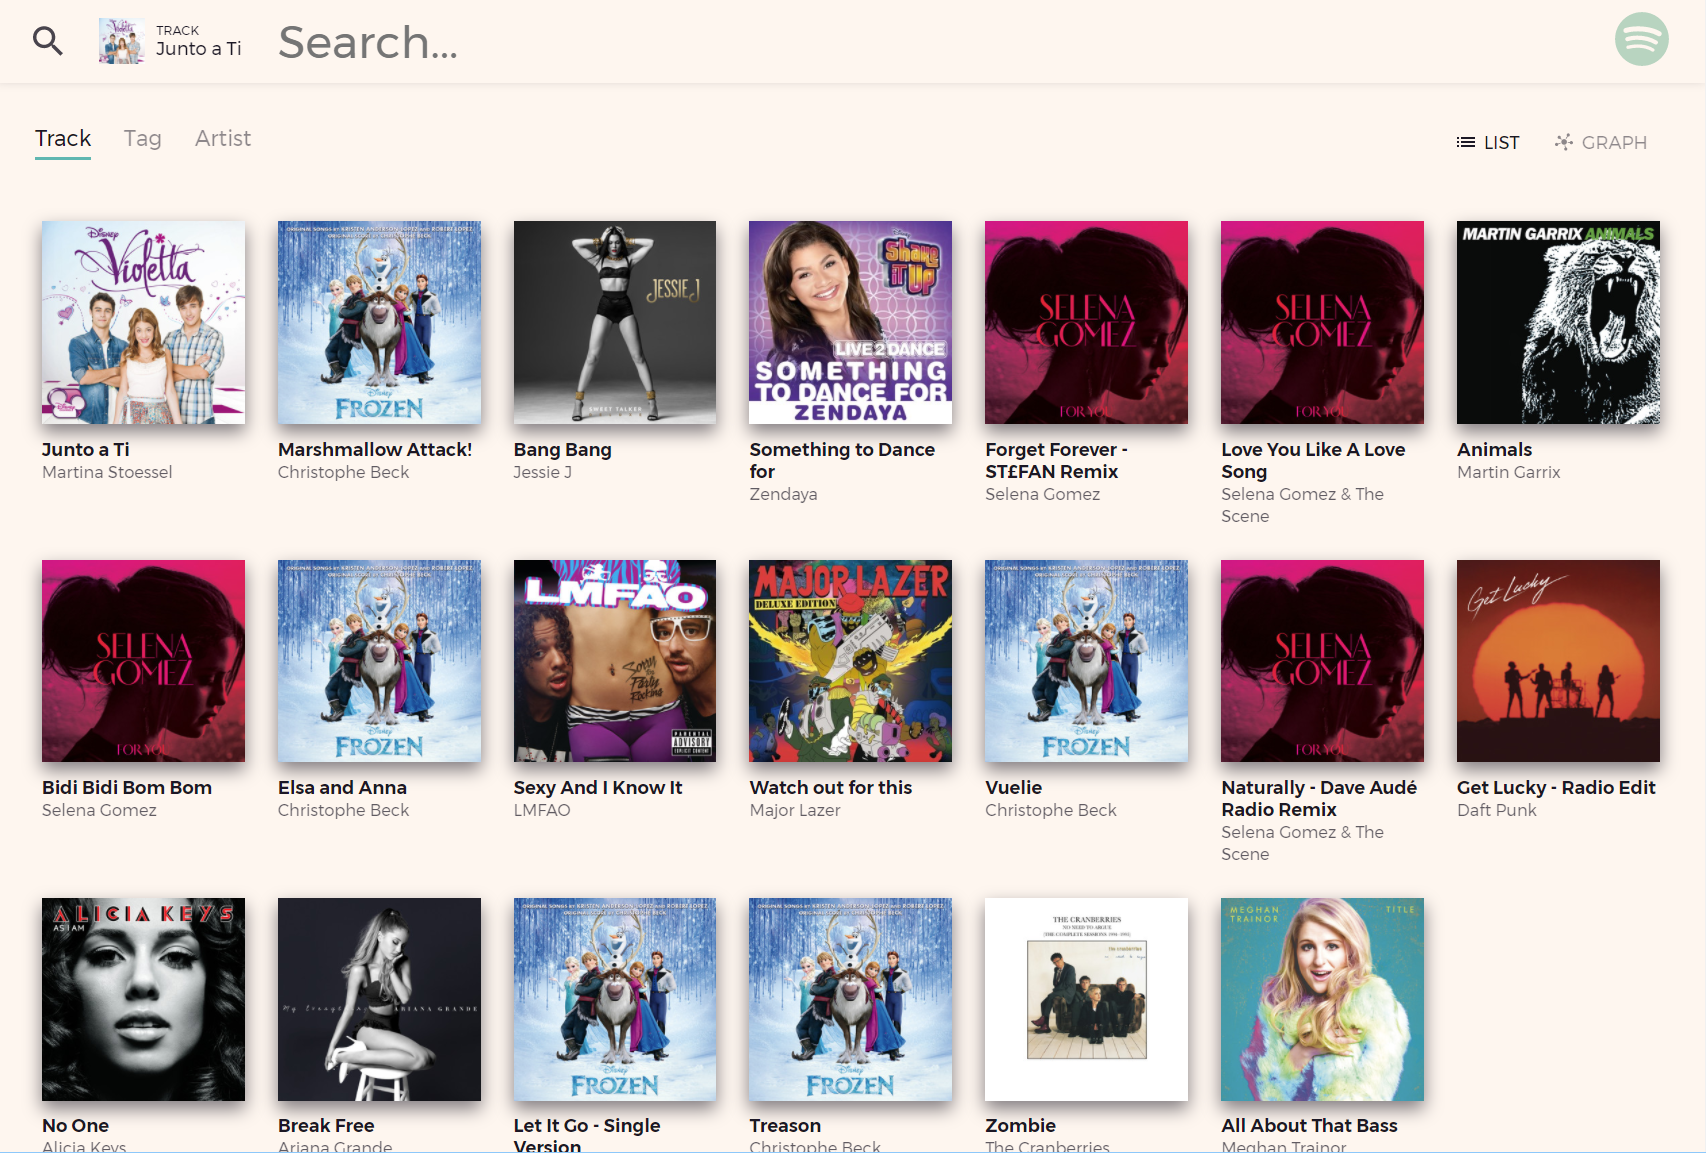
\includegraphics[width=200px]{web_client.png}}	
		\caption{Web client search suggestions}
		\label{fig:web_client}
	\end{figure}
	
	
	Search results are mostly displayed in list views to users. This representation has only the ordering as a one dimensional context information about the results. This is why the web client additionally implements a 3D view to view and explorer the search results.
	
	CLUSTER
	
	
	\subsection{Spotify connect}
	\label{sec:impl_spotify_connect}
	Initial dataset had only random users. To overcome the cold start problem and making the client usable, users can connect with their spotify account.
	
	User can connect with his Spotify account using OAuth. His music library is synced. Missing songs are added to the crawling list and later added to the graph. Then current embedding is extended to add user, possible additional songs and his preferences as user-track edges.
	Finally he can use the client with personalized results.
	
	
	
	Most Evaluation are based in offline ethods and lacking .... For online big dataset ist reqired. 
	
	Two challenges. Creating a Personal Profile (having Data + cold start). Andreas include new Users into model
	Spotify hast n usrres and is famius. Provides API with oauth connector
	Accessibg listening histoty ist possible but big  m and requres much more preprocessing and cimpitaional Power. 
	Tolassify User Stores music ist used instead. Tracks are ecplivity marked by User and modeling positive Feedback mich better. 
	
	After User authiruzed Access token ist used to sync music. Nö complete music Database -- compare eith Database. New Songs Mist be crawled -- fast, No huge dataset
	User needs to bei integrated into existing embedfing. Find new Songs and Users. Append as discussed in x. 
	
	
	
	System can only recommend known nodes. Getting better + icludes more tracks over time with users. Pretrained with Playlists as discussed in Evaluation. 
	
	\section{Experiments}
	Estimating the quality of the presented approach was one of the key challenges because there exist no dataset which directly maps search queries with user context to results. Even having a working prototype client to test the system on real users, representative user studies require fairly big and diverse users bases. The test cases somehow needs to allow the users to estimate the results without being biased through available options or the test environment. A/B test can model fair and solid results but require scopes in terms of number of users and participation which are only available on commercial platforms. Therefore the common approach in research is to make use of crawled playlists which were manually created by users. As presented in \cite{kamehkhosh2017user}, this evaluations are comparable to user studies but require much less effort. Additionally, offline experiments can be easily repeated with adapted implementations and input parameters which helps during implementation and optimization to observe and benchmark the outcome. \\
	
	Manually curated playlists can easily obtained, they have an user context and are usually labeled with a name. In a broader sense the contained tracks can therefore be seen as the desired output for queries by the name, related to the user. This is why the \emph{playlist evaluation}, further described in \ref{subsec:playlist_eval}, uses the playlists as ground truth and tries to predict the tracks based on user context and playlist name. To evaluate the embedding quality in respect to personal preferences the \emph{track recommendation evaluation} \ref{subsec:track_rec_eval} compares user track recommendations to baseline methods.
	
	
	\subsection{Dataset and graph generation}
	The initial dataset was constructed from a crawled Spotify playlists by DBIS [CITE]. This data consists of playlists with an user context and contained tracks with artist and audio features. In order to enrich the available query terms and gather more graph structure, social curated track tags were crawled from Last.fm \footnote{https://www.last.fm/api/show/track.getTags} and artist genres from Spotify.
	
	Table \ref{table:node_count} and \ref{table:edge_count} show which and how many elements and connections are contained in the graph.
	
	%% TODO: update numbers
	\begin{table}[H]
		\begin{minipage}{.5\textwidth}
			
			\centering
			\caption{Node count by type:}
			\label{table:node_count}
			\begin{tabular}{l|l}
				Playlists & 21,323  \\
				Users     & xxx     \\
				Tracks    & 671,903 \\
				Artists   & 83,789  \\
				Tags      & xxx
			\end{tabular}
			
		\end{minipage}
		\begin{minipage}{.5\textwidth}
			
			\centering
			\caption{Edge count by types (undirected):}
			\label{table:edge_count}
			\begin{tabular}{l|l}
				Playlist-User & 21,323  \\
				User-Tracks     & xxx     \\
				Track-Artists    & 671,903 \\
				Track-Tags   & 83,789
			\end{tabular}
			
		\end{minipage}
	\end{table}
	
	
	
	As expected, the more structural data is available the better the results perform, both for the \emph{playlist evaluation} and \emph{track recommendation evaluation}.
	
	\subsection{Playlist evaluation}
	\label{subsec:playlist_eval}
	For using the playlists as ground truth, known terms need to be extracted from the name as a first step. match with known terms and construct query. Using this terms a query can be constructed including the user. To evaluate the performance the IR measurements precision@k and recall@k are used.
	
	
	problems: many names are noisy and do not describe content in any sense. results are compared with random predictor.
	
	--> Query expansion
	
	% TODO: table with results
	
	% TODO: different methods for quering + query extraction
	
	% TODO: influence of embedding parameters: number of walks + dimensions
	
	\subsection{Track recommendation evaluation}
	\label{subsec:track_rec_eval}
	Queries are constructed using seeding elements combined with user context. Without seeds, the user alone can be used to query for recommendations. To perform a classic evaluation on user track recommendations, the playlists were used to construct historic track listening data, which is split into a training and test set. Using the test data, a new graph is generated and embedded. To compare the results, baseline scores are computed using \cite{Gantner2011MyMediaLite}.
	
	% TODO: table with results
	
	
	% TODO: describe results
	
	
	\section{Conclusion}
	This work presented an approach to use graph embedding techniques to create a low dimensional vector embedding of music data.
	
	
	% References
	\bibliographystyle{dbis}
	\bibliography{bibtex}
	
	
\end{document}
